\FloatBarrier
\chapter{Implementation}

The following chapter describes the implementation of miq.
Miq is the program that was developed as a proof of concept
of the topics described in this document. As such, miq
(pronounced [miku]), is a package manager for Linux. It can
be categorized as a ``source-based'' package manager,
because the user would build every package from its sources
(for example, Gentoo's package manager |emerge| or |nix|),
as opposed to to a ``binary-based'' package manager, which
distributes the already-built packages to its users.

The model of a source-based package manager provides some
advantages, such as being able to edit the recipes that
build the packages. Moreover, by integrating the tool that
builds the packages and the tool that installs them, the
user gets a fast feedback loop to iterate over the writing
of the package definitions. In a source-based package
manager, the user receives a copy of a source tree that
contains the recipes, definitions of all the packages in the
repository. These files contain the instructions about all
the packages that are available, and the machine-readable
data for the package manager to build them. The user would
tell the package manager to build or install certain package
X, and the program would then:

\begin{itemize}
    \item Evaluate the file tree of package definitions.
    \item Calculate a transaction (which files to build or download)
    \item Perform the transaction
\end{itemize}


miq is heavily inspired by nix, the functional package
manager, a work of \Citeauthor{dolstraNixOS2008}
\cite{dolstraNixOS2008}. The work of nix of using a
hash-based path system instead of the \ac{FHS} was the idea
that lead this project, and that is implemented in miq by
following the same conventions that in nix. This means, that
packages are configured with a custom prefix that lives in
the \textbf{store} (|/miq/store| and |/nix/store| respectively), with
a unique subdirectory based on the hash of the package
definition -- which implies that any change in its
dependencies would trigger a recalculation of the store
path. Miq differs with nix in that the schema for the
calculation of the store path follows the pattern
|name-version-hash|, while nix uses |hash-name-version|.
While the result of the package is functionally the same, by
using the name first, the list of folders in |/miq/store|
can be easily ordered by package name.

Miq differs from nix in the usage of the language used for
the evaluation of the packages. On of the powerful features
of both miq and nix is the ability to declare packages as
code, using a turing-complete programming language. This is
in contrast to apt or rpm, which use a markup language to
define the packages. By using a turing-complete language,
the user is able to create any kind of abstraction around
the package primitives. This not only allows for code
deduplication, but also to easily create new ``helper''
packages that would otherwise not be considered with a
classical markup-language based package manager.

In this regard, for nix, a new programming language was
invented with the same name, nix. This is a purely
functional language inspired by the semantics of Haskell, and
often referred to as ``JSON with functions''. As this
language is sometimes alien to users, with miq the decision
was to use Lua, an easily emendable language. This is
discussed in more depth in section \ref{sec:lua} .

Miq is implemented in the Rust programming language
\cite{RustProgrammingLanguage} . Rust is a relatively new
language created at Mozilla, which focuses on the ability to
build fast and reliable programs. This is achieved through
the use of rich type system, that guards the programmer from
making mistakes and eases the process of a refactor. Rust
also provides some other features that were viable to this
project. A very important detail is that Rust can build
native binaries (ELF) that can be run by the operating
system. Every dependency of the Rust program (crates) are
also built into the final binary, and C library requirements
(libc) are statically linked. This means that the final
result is a single |20MB| binary, with no dependencies that can be
run in any Linux system, no matter the distribution.

\section{Units: the basic building blocks}
\label{sec:unit}

The main purpose of the package manager, is to build
packages according to a dependency tree. Therefore, it is
important to properly define what a ``package'' is and is
not. In miq, the concept of a package has been abstracted by
the concept of a ``unit''. A unit is something that can be
built, and put into the miq store (|/miq/store|). This
abstraction has been chosen, because it makes it easy to
have different entities that can be built. This
differentiation serves the purpose of being able to declare
2 types of units: package units, and fetchable units.
As discussed in section \ref{sec:builder}, package units are
built in a network sandbox, to avoid impurities resulting of
a connection to the network. The main aspect of miq is being
able to hash packages depending on its dependencies and
build script. The ``result'' of building the package is not
considered in the hashing algorithm. This can be described
as packages being input-addressed, instead of
content-addressed. As such, it is important to have a proper
build sandbox to isolate the build process and produce a
reproducible result, for the same input parameters. The
purpose of fetchable units (|Fetch|) is to be able to split
the network connection from the build process. The
implementation for |Unit| is a enumeration with 2 cases:

\begin{minted}{rust}
#[derive(Clone, Debug, Serialize, Deserialize, Hash)]
enum Unit {
    PackageUnit(Package),
    FetchUnit(Fetch),
}
\end{minted}

This example already shows one of the features of Rust that
made the development of miq ergonomic: |derive| macros.
|derive| is a keyword that allows for automatic code
generation given some |struct| or |enum|. In this case the
|Hash| trait is derived. What this means is that Rust
automatically generates an implementation for the |Hash|
trait, given that the fields of the enum are also |Hash|.

Very importantly too, the traits |Serialize| and
|Deserialize| are derived for Unit. These traits are
provided by the |serde| crate (serialization and
deserialization) \cite{Serde} . Similarly to the |Hash|
derive macro, serde allows to automatically generate
serialize and deserialize a Unit from any crate that
provides an interface for it. This comes into play for the
usage of the intermediate representation objects that are
store into disk, in |toml| format. As discussed in the next
section, miq loads the units from disk in |toml| format, and
automatically parses them into the data structure, without
any need of parsing code.

The Unit enum has two members, which wrap the inner values:
|Package| and |Fetch|. These are structs that contain all
the information that miq uses to build the Unit. The
implementation of the Fetch unit is trivial, as the
following code snippet shows:

\begin{minted}{rust}
#[derive(Deserialize, Serialize, Hash)]
struct Fetch {
    result: MiqResult,
    name: String,
    url: String,
    executable: bool,
}
\end{minted}

The toml format is an human-readable serialization format,
that can be compared to JSON. As the latter is not
considered ergonomic to manually write, it was decided to
use the toml format instead, although this doesn't have any
impact on the functioning of the package manager. The
following snippet of code shows a serialization of the musl
Fetch Unit.

\begin{minted}{toml}
# /miq/eval/musl-1.2.3.tar.gz-828bf8f78328fb26.toml
type = "FetchUnit"
result = "musl-1.2.3.tar.gz-828bf8f78328fb26"
name = "musl-1.2.3.tar.gz"
url = "https://musl.libc.org/releases/musl-1.2.3.tar.gz"
executable = false
\end{minted}

The example above already shows the hashing of the Unit
itself: the |result| field. This field is computed as a
function of the |url| and the |executable| fields, and
determines the hashing of the Unit itself. This is stored
attached to the Unit itself. This example is trivial, but
any other Fetch unit with the same |name|
(|musl-1.2.3.tar.gz|) but different |url|, would trigger a
change in the hashing that ends up in |result|, as shown in
figure \ref{fig:fetch_hash} .

\begin{figure}[hbt]
    \centerfloat
    \includesvg[width=350pt]{assets/fetch_hash.svg}
    \caption{Hashing process of a Fetch Unit.}
    \label{fig:fetch_hash}
\end{figure}

Similarly, a Package Unit is written as a struct with the
instructions required to build it. The following simplified
snippet shows the implementation in Rust:

\begin{minted}{rust}
#[derive(Serialize, Deserialize, Hash)]
pub struct Package {
    result: MiqResult,
    name: String,
    version: Option<String>,
    deps: BTreeSet<MiqResult>,
    script: String,
    env: BTreeMap<String, String>,
}
\end{minted}

An example serialization of a Package Unit for musl is the
following:

\begin{minted}{toml}
# /miq/eval/musl-f0dd14ee1ca91c64.toml
type = "PackageUnit"
result = "musl-f0dd14ee1ca91c64"
name = "musl"
version = "1.2.3"
deps = [
    "musl-1.2.3.tar.gz-unpack-5f9d5116c4c83592",
    "stage0-stdenv-d2ecc89c54b1b316",
]
script = '''
source /miq/store/stage0-stdenv-d2ecc89c54b1b316/stdenv.sh
set -ex
/miq/store/musl-1.2.3.tar.gz-unpack-5f9d5116c4c83592/configure \
    --prefix=$PREFIX \
    --disable-static \
    --enable-wrapper=all \
    --syslibdir=$PREFIX/lib
make -j$(nproc)
make -j$(nproc) install
ln -vs $PREFIX/lib/libc.so $PREFIX/bin/ldd
'''
\end{minted}

A Package Unit is more complex than a Fetch Unit, because of
the following:
\begin{itemize}
    \item Package units have a |deps| field. |deps| are the
    |result| strings of any other Unit. This means Package
    Units can depend on other Package or Fetch Units, while
    Fetch Units don't depend on anything.
    \item The |build| field is a literal bash script that is
    used during the build process to produce the output.
\end{itemize}

In contrast to other package managers and similarly to nix,
miq doesn't provide multiple stages for the build process.
In Gentoo, the definition of package, usually contains some
unpack, build and install phases. In contrast, everything in
miq is done through the script section. This is because, by
using a language to generate this |toml| representation, the
user is free to include any custom functionality as needed.
This is important, as the Package Unit tries to be as
minimal as possible, by just providing the |script| phase,
and letting the user construct any abstraction on top of it.
In the example, musl depends on |stdenv| (standard environment), which is a script
that sets some environment variables required for the build
process, effectively implementing the concept of build
stages in other package managers.

\begin{figure}[hbt]
    \centerfloat
    \includesvg[width=350pt]{assets/phash.svg}
    \caption{Hashing process of a Package Unit.}
    \label{fig:pkg_hash}
\end{figure}

The hashing algorithm used for the process is the
\textit{Fowler Noll Vo} hash function \cite{FnvRust}. While
this algorithm is not cryptographically secure, and doesn't
provide protection against collision attacks, the algorithm
could be considered as sufficient for this application. This
could be considered as an implementation detail, and could
be swapped for any algorithm such as |SHA256| if deemed
necessary.

The implementation of miq uses a 2-stage evaluator, that
first converts the Lua code into a serialization of Units,
and then serializes them again to sort the dependency
algorithm. Unit files are stored in the |/miq/eval|
directory, generated and consumed by miq in sequence, as
shown in figure \ref{fig:2stage} .

\begin{figure}[hbt]
    \centerfloat
    \includesvg[width=400pt]{assets/22stage.svg}\
    \caption{Two-staged evaluation process.}
    \label{fig:2stage}
\end{figure}

The purpose of this 2-stage evaluator process, is be able to
extend miq as needed. Because the |unit.toml| format is
well-known, a user or contributor should be able to
implement a different evaluator in any other language than
Lua. This is one of the main shortcomings of nix, as it
only allows the usage of the nix language. The Guix package
manager \cite{courtesFunctionalPackageManagement2013}
studied the usage of Scheme as the language for the
evaluation process, by patching into the nix builder. By
explicitly allowing for an intermediate format, the
ergonomics of the package manager could be improved.

As a side-effect of this design, some characteristics
emerge:

\begin{itemize}
    \item Units toml files can be manually written by hand.
    During the development process of miq, the Lua evaluator
    was the last piece implemented, because Unit files could
    be manually written as a proof of concept.
    \item Units can be copied and pasted from one machine to
    another. If the reproducibility of the evaluator cannot
    be assured, unit files can be checked out into version
    control. A user could then use the locally downloaded
    unit tree to build the resulting packages. This could be
    useful as an alternative distribution method to the Lua files.
\end{itemize}

\section{Dependency solver}

The package dependencies are evaluated by constructing a
\acl{DAG} on memory, by reading the intermediate
representation Unit files in |toml| format. As mentioned in
the previous chapter, a Unit is an abstraction over what a
package is, that stores the instructions to perform the build
or fetch process. The \ac{DAG} is
composed of edges of no weight and nodes that are weighted
with Unit's (after being deserialized). The root unit it
selected by the user via the \ac{CLI}. The process to
construct the graph is the following:

\begin{enumerate}
    \item Start at node $N$ with some Unit weight
    \item Read the node's dependencies into a list of Nodes
    \item For each child node $N'$
    \begin{enumerate}
        \item Search the graph for $N'$, and add it if it is
        not present
        \item Add an edge from the child to the parent, such as $N <- N'$
        \item Recursively perform the algorithm for this
        child node
    \end{enumerate}
\end{enumerate}

This recursive process recursively performed, until one of
the branches reach a Fetch Unit. Fetch Units don't have
dependencies, so the stack returns and unfolds into the
parent task that called it. A visual representation of this
process is illustrated in figure \ref{fig:depbuild} .

\begin{figure}[hbt]
    \centerfloat
    \includesvg[width=300pt]{assets/dep_build.svg}
    \caption{Process to build the dependency graph.}
    \label{fig:depbuild}
\end{figure}

More in detail, the process that walks the children of a node
performs the following computations:

\begin{enumerate}
    \item Read the |deps| field of (Package) Unit node.
    |deps| is implemented as a |Vec<MiqResult>|. |MiqResult|
    is a type-alias for a |String|, such that it can safely
    be handled in the proper scenarios. A |MiqResult|
    contains the portion of the store path |<name>-<hash>| .

    \item The |MiqResult| is converted into a |MiqEvalPath|
    . The evaluation paths points into the file that
    produces the Unit, it can be considered a pointer to the
    Unit. This means it is converted to the shape
    |/miq/eval/<name>-<hash>.toml| .

    \item The toml file contained in the |MiqEvalPath| is
    automatically serialized into a Unit, as explained in
    section \ref{sec:unit} .
\end{enumerate}

The \ac{DAG} is stored in memory by creating a mapping of
Node ids to Units. To store the edges, it is used a mapping Node ids to
Node ids 1-to-1, such that direction is preserved. The Rust
crate ``daggy'' \cite{DaggyRust} is used to provide this
data structure, and the required methods to manipulate the
graph, such as reading or writing nodes and edges. On the
type level, it is
constructed a simple type alias to store the result:

\begin{minted}{rust}
type UnitDag = daggy::Dag<Unit, ()>;
\end{minted}

\section{Package definitions and Lua evaluator}
\label{sec:lua}

Miq is a source-based package manager, which means that the
user downloads a copy of a source tree, which includes all
the definitions for all the packages. These definitions
contain the instructions for the package manager to build
the package into the user's disk. In contrast, a binary-based
package manager has a list of just the packages available
(usually in the form of a database that is synced -- |apt update|), and the user downloads the already built packages
from the distribution's servers.

Miq's deployment model, similarly to Nix's, is to have each
definition of a package reference the exact paths of its
dependencies. A Unit, the intermediate representation of a
package definitions, contains a |deps| field, which lists the
packages by its hashed name, and the |script| field may
contain hardcoded paths to these packages. The following
example shows these hardcoded paths:

\begin{minted}{toml}
# /miq/eval/musl-f0dd14ee1ca91c64.toml
type = "PackageUnit"
result = "musl-f0dd14ee1ca91c64"
name = "musl"
version = "1.2.3"
deps = [
    "musl-1.2.3.tar.gz-unpack-5f9d5116c4c83592",
    "stage0-stdenv-d2ecc89c54b1b316",
]
script = '''
source /miq/store/stage0-stdenv-d2ecc89c54b1b316/stdenv.sh
set -ex
/miq/store/musl-1.2.3.tar.gz-unpack-5f9d5116c4c83592/configure \
    --prefix=$PREFIX \
    --disable-static \
    --enable-wrapper=all \
    --syslibdir=$PREFIX/lib
make -j$(nproc)
make -j$(nproc) install
ln -vs $PREFIX/lib/libc.so $PREFIX/bin/ldd
'''
\end{minted}

The purpose of the package evaluator is to resolve these
paths in a step before the build process. A user does not
use the paths directly, as they are calculated by miq. By
using an scripting language, the user would be able to
declare the dependencies in a programmatic way.

To do so, miq uses the Lua programming language. The
previous Unit definition is compiled from the following Lua
code (simplified):

\begin{minted}{lua}
do
    local version = "1.2.3"
    local src = x.fetchTar {
        url = f "https://musl.libc.org/releases/musl-{{version}}.tar.gz",
    }
    x.libc = x.stdenv {
        name = "musl",
        version = version,
        script = f [[
            {{src}}/configure \
                --prefix=$PREFIX \
                --disable-static \
                --enable-wrapper=all \
                --syslibdir=$PREFIX/lib
            make -j$(nproc)
            make -j$(nproc) install
            ln -vs $miq_out/lib/libc.so $miq_out/bin/ldd
        ]],
    }
end
\end{minted}

By using a scripting language to build the intermediate
representation, the absolute paths used by miq are
abstracted away from the user, while still allowing for this
filesystem model.

The previous Lua example shows the usage of some functions
built specifically for miq. To begin with, the |f| function
is analogous to f-strings in Python, where one can insert
the string representation of a variable into a string. This
|f| function is exported by the |miq| library, which
executes in Rust, and is automatically inserted into the
runtime of the script executing, by using a |require|:

\begin{minted}{lua}
local miq = require("miq") -- added by the Rust runtime
local f = miq.f

local a = 1
local b = f("a is {{a}}") -- => "a is 1"
local c = f "a is {{a}}" -- => "a is 1" (different function calling syntax)
\end{minted}

|f| is implemented using Lua's debugging facilities, which
comes with its drawbacks. The main issue is no editor knows
about the custom syntax for a string (using the |{{}}|
pattern), which means that the editor is not able to warn
the user about a syntax error.

More importantly, the |f| function not only is able to
interpolate strings into strings, as shown in the previous
snippet, but it is also able to interpolate Units. To create
a Unit, a user is able to use the |miq| library to create a
unit. By providing a user input, the fields are hashed and
converted into a Unit, which then is serialized into a Lua
table. The table is the only data structure in Lua, and
holds a mapping of keys to values.

\begin{minted}[obeytabs=true,tabsize=2]{lua}
local miq = require("miq")

local toybox = miq.fetch {
	url = "http://landley.net/toybox/bin/toybox-x86_64",
	executable = true,
}
--[[ => {
  executable = true,
  name = "toybox-x86_64",
  result = "toybox-x86_64-69a4327d80d88104",
  type = "FetchUnit",
  url = "http://landley.net/toybox/bin/toybox-x86_64"
}
--]]
\end{minted}

When |f| is used to interpolate a Unit, instead of returning
a new string, it returns a custom type called |MetaText|. A
|MetaText| is a wrapping type around a string, that also
holds the packages that depend on this text, with the
following Rust type signature:

\begin{minted}{rust}
struct MetaText {
    value: String,
    deps: Vec<MiqResult>,
}
\end{minted}

By interpolating a Unit into a string, the resulting
|MetaText| is used to carry the packages that ``depend'' on
this text. Instead of the user having to manually declare
what dependencies are needed for the package, they can just
directly interpolate the package into a MetaText, and the
information about the dependency is carried over. The result
of interpolating a Unit into a MetaText, is the store path
of the unit (|/miq/store/name-hash|), as shown in the
following Lua snippet:

\begin{minted}{lua}
local miq = require("miq")
local f = miq.f
toybox = miq.fetch {
    url = "http://landley.net/toybox/bin/toybox-x86_64",
    executable = true,
}

local t = f "ls -la {{toybox}}"
--[[ => {
  value = "ls -la /miq/store/toybox-x86_64-69a4327d80d88104",
  deps = { "toybox-x86_64-69a4327d80d88104" }
}
--]]
\end{minted}

Putting everything together, the |f| functions allows the
user to:

\begin{itemize}
    \item Declaratively define the relationships between packages.
    \item Abstract away the absolute paths used by miq, in
    the context of shell scripts.
    \item Automatically append the interpolated packages
    into the dependencies of a package.
\end{itemize}

The usage of Lua as a programming language for scripting the
package definitions comes down to the fact that the language
can be completely embedded into the Rust application. By
using the |mlua| crate \cite{MluaRust} . This library allows
to embed a complete Lua runtime inside a Rust application,
and provides a safe interface to interact with it. Instead
of using any other scripting language like Python, and
relying on message passing and subprocess execution, the Lua
runtime is able to directly communicate with the Rust code
by sending and receiving data. The Rust code is able to call
Lua functions, and the Lua code is similarly able to call
Rust functions easily. While Lua is a dynamically typed
language , the |mlua| crate provides type safety to the
received values, and is able to serialize and deserialize
Rust types into Lua tables. This seamless integration
between the two languages allows for an application written
in an ergonomic language for a big project, while letting
the user the flexibility of a scripting language for the
declaration of the packages.

As a result of using a scripting language to declare the
packages, the writer of the package tree is able to abstract
away common components into smaller functions. Instead of
having to write some boilerplate code around the primitives
(|miq.f|, |miq.package| and |miq.fetch|), one is able to
write ``wrappers'' around the built-in functions. This
allows for a more ergonomic experience around the
primitives, and extension of the functionality.

For example,
the primitive |miq.fetch| creates a Fetch Unit from its
input. A Fetch Unit is simply fetched from the internet, and
stored into the filesystem. Very commonly, this Fetch is a
tarball that the package script unpacks to build it. So, a
wrapper around |miq.fetch| can be created, such that it
creates an intermediate package that unpacks the tarball.
To implement this in Lua:

\begin{minted}[obeytabs=true,tabsize=2]{lua}
fetchTarBuilder = function(input)
    local input = input

    local fn_result = function(args)
        local args = args
        local input = input
        local post
        if args.post ~= nil then
            post = args.post
        else
            post = "# No post unpack"
        end
        local fetch = miq.fetch(args)
        local pkg = miq.package {
            name = f "{{fetch.name}}-unpack",
            script = f [[
                set -ex
                export PATH="{{input.PATH}}"
                cd $miq_out
                tar -xvf {{fetch}} \
                    --strip-components=1 \
                    --no-same-permissions \
                    --no-same-owner

                {{post}}
            ]],
        }
        return pkg
    end
    return fn_result
end

fetchTar = fetchTarBuilder {
    PATH = f "{{bootstrap}}/bin",
}

fetchTar {
    url = f "https://musl.libc.org/releases/musl-{{version}}.tar.gz",
}
\end{minted}

As can be seen, the |fetchTar| uses some base package that
provides the |tar| executable (in this case from the
|bootstrap|) package to unpack the input url, by using a
Fetch Unit, and a Package Unit that depends on it. While Lua
is not the most powerful language, it allows for some
abstractions over the primitives.

Finally, it should be noted how miq knows what file to
evaluate in the first place. The user is able to provide a
path to either a Unit file (|/miq/eval/name-hash.toml|) or
to a Lua file. If the file extension is |.toml|, then the
Unit is directly read, skipping the evaluator phase directly
into the intermediate representation and dependency
evaluator. Otherwise, the file is take as the ``top-level''
Lua file. The top-level file should return a table, and the
user is able to select which item to build from it. For
example, if the user select the reference
|./pkgs/init.lua#foo|, then |init.lua| is completely
evaluated, and the |foo| key is selected from the resulting
table. This method of references to files with different
extensions could be extended to any other scripting language
used to evaluate the packages, with minimal changes to the
\ac{CLI} parser.


\section{Builder}
\label{sec:builder}
As mentioned in previous sections, miq has a 2-stage package
evaluator that produces a dependency graph of Units in
memory. This dependency graph is consumed during the build
process, executing the script of each Package Unit or
fetching the necessary files of Fetch Units.

\subsection{Sandbox}

Fetch Units are trivially built, as it is only needed to do
an http request to the selected |url|, and store the
resulting file into the store path. Optionally, the user
might select to change the permissions of the file to be executable.

Package Units use a more involved process. To begin with,
they are built in a build sandbox. The purpose of the
sandbox is to isolate the execution of the script from the
outside world. This means that the process only sees a
limited view of the filesystem and network connection is
limited. The sandbox isolates the filesystem by only giving
the process views on essential paths, like |/dev|, |/proc|
or |/tmp|. A view on |/miq/store| is also allowed, and the
build scripts contain absolute paths into it. For this
reason, it does not matter what the existing content of the
store is from one machine to another, as only the
``hardcoded'' paths into the dependencies are used. The
development model of miq by hashing every package to provide
a unique path completely bypasses the need to selectively
mount specific packages into the build sandbox. To create
this sandbox, miq relies on Linux namespaces
\cite{NamespacesLinuxManualb} . Linux namespaces are an
interface provided by the kernel itself, to change
resources of a process. The resources that can be changed
include: mount points, user ids, network, etc. While
initially miq leveraged directly the namespaces interface
via the |libc| crate, it was later changed to run the
program bubblewrap as a subprocess . Bubblewrap \cite{Bubblewrap2023} is a C
application that wraps the namespaces interface with a
\ac{CLI}, such that the user can easily run processes in a
sandboxed environment. Therefore, miq calls bubblewrap with
the appropriate flags to provide a build sandbox for the
build script.

The usage of a sandbox is crucial for the reproducibility of
the package builds. The development model of miq assumes
that a package is uniquely identified by its hash, which in
turn is derived from its inputs (build script and
dependencies). If the package produces a result that is not
reproducible, this means that a same hash potentially points
to different results -- from one computer to another or
rebuilds in the same computer. Some of the sources of
``impurity'' are:

\begin{enumerate}
    \item Environment variables
    \item User id, name and groups
    \item Files that are not part of the miq store, like
    |/etc|, |/home|, |/var|, etc.
    \item Network connection (e.g. fetching from the
    internet might fail or give different results)
\end{enumerate}

Environment variables are trivially cleaned by any
subprocess invocation. Miq additionally inserts some extra
environment variables, like |\$miq_out|, which points into
the output directory or |\$HOME| pointing to the build
directory.

To isolate the user id, user namespaces are used. User
namespaces allow to create a mapping of user ids outside the
sandbox into user ids in the sandbox. In practice, the user
running miq is mapped into the root user. The child process
``sees'' that it is running as root, while it is being
executed on behalf of the user (with all the limitations and
permissions of the user, not of root).

The filesystem can be isolated by using a mount namespace.
It allows to mount a new root |/|,
and then selectively mount the necessary paths into this
blank slate. Some core paths are required, such as |/dev| or
|/proc| to even be able to run any application. A mapping of
a build directory into the sandbox at |/build| is created.
It is also possible to mount |/miq/store| as read-only, such
that the build script is not able to modify any existing
package by accident.

Finally, the network connection can be trivially
disconnected by using network namespaces and the appropriate
flags to bubblewrap. As mentioned before, Fetch Units are
not built in a sandbox and rely on fetching files from the
internet, which can potentially produce impure,
non-deterministic results. This can be avoided by using a
resource-integrity mechanism
\cite{chapuisEmpiricalStudyUse2020} . What this would
involve is checking that the received content matches
against an already-known hash, that is derived from the file
contents. The hash can be manually calculated by \acl{TOFU}
and written in the package definition. This is currently not
implemented into miq, but it is a planned feature.

\FloatBarrier
\subsection{Concurrency}
\label{sec:concurrency}

As the source-based package managers NixOS's nix and
Gentoo's emerge, miq is able to build package in parallel. A
parallel build process implies that there the build is not
sequential. In a sequential (or 1-job build), every package
is built one after the other, waiting for the previous in
the line to build the next one. Considering that the
structure used to represent the dependency graph is a
\acl{DAG}, on first iteration one solution is to compute the
topological sort of the graph
 . This sort
involves converting the graph into a sequence of nodes, such
that the ordering between the nodes is preserved
\cite{erParallelComputationApproach1983} . Finally, a
builder can travel the sequence to build each dependency in
order on after the another.
This process is not efficient, as a package only requires
that its dependencies are built, but not every node in the
topological sort. Figure \ref{fig:toposort} shows an example
of a topological sort of a simple package that depends on 2
Fetch Units. In this situation, only when one of the Fetch
Unit finalizes the transaction, which involves downloading
the file from the internet and saving it to the disk, can
the next Fetch Unit start its process.

\begin{figure}[hbtp]
    \centerfloat
    \includesvg[width=280pt]{assets/toposort.svg}
    \caption{Topological sort of a \ac{DAG} with 2 Fetch Units.}
    \label{fig:toposort}
\end{figure}

A more complex example of how a topological sort is not
desired is shown in figure \ref{fig:toposort2} . As can be
seen, Package B must wait until Fetch B has finished, while
all its dependencies (just Fetch A) has already been built.
Similarly, Package C must wait until Package B has been
built. As a result of the definition of a topological sort
being a sequence of nodes where ordering is respected, all
the edges in the topological sort point ``upwards'' into the
root unit. Cyclic graphs cannot be topologically sorted, as
the ordering cannot be preserved, and we would need to build
a package as a dependency of itself, as displayed on figure
\ref{fig:toposort3} .

\begin{figure}[hbtp]
    \centerfloat
    \includesvg[width=300pt]{assets/toposort2.svg}
    \caption{Topological sort of a \ac{DAG} with 2 Fetch and
    2 Package Units.}
    \label{fig:toposort2}
\end{figure}

\begin{figure}[hbtp]
    \centerfloat
    \includesvg[width=300pt]{assets/toposort3.svg}
    \caption{Impossible topological sort of a directed cyclic graph.}
    \label{fig:toposort3}
\end{figure}

\FloatBarrier

A builder that uses topological sort can be easily
implemented, as the library that provides the \ac{DAG}
structures also provides the method in
|daggy::petgraph::algo::toposort|. While miq used this
sequential approach initially, it was developed a new
algorithm to perform the builds concurrently. To properly
track the Units that have been built or not, the following
|enum| is used:

\begin{minted}{rust}
enum BuildTask {
    Waiting,
    Building,
    Finished,
}
\end{minted}

To begin with, every Unit gets attached a new |BuildTask| by
creating a simple map of the list of Units to their state.
Every Unit starts in the |Waiting| state.

\begin{minted}{rust}
let mut build_tasks: HashMap<&Unit, BuildTask> = HashMap::new();
\end{minted}

Then, an iterative process is started, following the steps:

\begin{enumerate}
    \item Scan all the Units in the \ac{DAG}. For every Unit U do:
    \begin{enumerate}
        \item Scan all of U's dependencies. If all of them
        are |BuildTask::Finished|, or if there are no dependencies,
        then U can be built.
        \item Spawn a new thread to build U, and mark it as
        |BuildTask::Building| in the map.
    \end{enumerate}
    \item Wait for any thread to finish. If the tasks is OK,
    mark it as a |BuildTask::Finished|. If any errors occur,
    return them and stop any other tasks.
    \item If all tasks are |BuildTask::Finished|, return.
    Otherwise loop back to the first step.
\end{enumerate}

Overall, the algorithm scans the \ac{DAG} in a infinite
loop, spawning ne threads to build the Units, as soon as
they can be built. This happens when all of a Unit's
dependencies have finished.

Rust's asynchronous ecosystem is leveraged to be able to
spawn threads that don't block. The asynchronous runtime
used for this task is Tokio \cite{TokioRust}, as the Rust
language only provides the primitives to declare
asynchronous functions on the type level, but doesn't
provide any runtime to execute them. Tokio and the async
Rust ecosystem is based on the concept of green thread. A
green thread is a thread that is not executed by the
operating system, but rather by a runtime (in this case,
Tokio). A green thread runtime uses its available CPU time
to context-switch between a list of tasks that are waiting.
Whenever a task is being executed, it is the only task that
the runtime executes -- without any parallelism -- until the
task hits an |await| point. Then, the runtime switches the
context to another tasks that is waiting, until that one
also hits an await point. The process is repeated until all
tasks have finished. Thus, the runtime is only executing a
single task at any instant of time, but the context
switching between tasks provides the illusion of the tasks
being executed in parallel, as shown in figure \ref{fig:timeshare} .

\begin{figure}[hbt]
    \centerfloat
    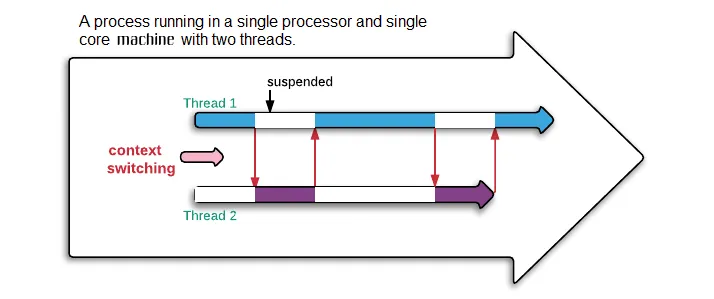
\includegraphics[width=350pt]{assets/timeshare.png}
    \caption{Context switching between tasks in a green thread runtime.}
    \label{fig:timeshare}
\end{figure}

Tokio also provides a hybrid approach to threads, as it uses
a thread pool to execute the tasks. The thread pool is
mapped into operating system threads, so the tasks can be
run in parallel if the runtime decides to put them into a
different backing \ac{OS} thread.

However, a parallel runtime is not needed for miq, as the
build tasks are spawned as a subprocess for bubblewrap, the
build sandbox discussed in the previous subsection. Every
tasks executes bubblewrap, which gets a new \acl{PID} and is
executed by the OS apart from the thread runtime. Thus, the
tasks executed by miq only collect the logs generated by the
bubblewrap subprocesses, which happens concurrently.

\begin{figure}[hbt]
    \centerfloat
    \includesvg[width=350pt]{assets/parallel.svg}
    \caption{Concurrent process to build 5 Units.}
    \label{fig:parallel}
\end{figure}

Figure \ref{fig:parallel} shows an example of how this
algorithm schedules the builds such that every Unit is built
as soon as every dependency has been built. The colors for
the figures indicate:
\begin{itemize}
    \item White: |BuildTask::Waiting|
    \item Yellow: |BuildTask::Building|
    \item Green: |BuildTask::Finished|
\end{itemize}

The process is as follows:

\begin{enumerate}
    \item Units E and D have no dependencies, so they are built first.
    \item D finishes, so C can be built now. A build task is
    spawned for C.
    \item E finishes, which was required along D for E. E
    starts building.
    \item When both B and C have finished, the last node A
    can be built.
\end{enumerate}


\FloatBarrier
\subsection{C flags and package configuration}

The deployment model of miq is based on not using the
\acl{FHS} as a basis of the install locations, but rather
using unique prefixes for every package. These prefixes are
calculated at evaluation-time, and are based on the package
(Unit) definition and dependencies, such that a unique
prefix is generated for each Unit. This prefix is calculated
with a hashing function, and is used as the root directory
for the installation of the package. For this reason,
packages in miq must be configured to use this path, which
is available during the build process as the |\$miq_out|
environment variable, and substitutes |/usr| in a
traditional Linux package manager. The following mappings of
paths are used:

\begin{figure}[hbt]
    \centerfloat
    \begin{tblr}{hlines, vlines}
        /usr/share & /miq/store/name-hash/share \\
        /usr/lib  & /miq/store/name-hash/lib \\
        /usr/bin  & /miq/store/name-hash/bin \\
        /usr/include & /miq/store/name-hash/include \\
    \end{tblr}
    \caption{Mapping of \ac{FHS} paths to miq store paths.}
\end{figure}

To properly produce C binaries that use this paths, it is
imperative to use a correct set of flags for the compiler
and linker. As mentioned in the previous chapter in section
\ref{sec:elf-format}, Linux uses the \acl{ELF} format for
binary files. \ac{ELF} files contain some metadata about the
file distributed in different sections, and also the
assembly itself. The metadata is used by the Linux kernel to
properly load the executable into memory. For a dynamically
linked \ac{ELF} -- statically linked \ac{ELF}'s are not
distributed in Linux operating systems unless needed -- the
Linux kernel first needs to read the \acl{PHT} looking for
the |INTERP| entry. This is the ``link loader'', a program
provided by libc which handles the rest of the loading
process. On a conventional distribution, |INTERP| points
into |/lib64/ld-linux-x86-64.so.2| and this is compiled into
the executable without any special flags.

To be able to change the link-loader that is written to the
executable, a flag \cite{GNUCompilerCollection} can be
passed ot the linker by using the |-dynamic-linker| flag:

\begin{minted}{text}
gcc -Wl,-dynamic-linker=/miq/store/libc-hash/lib/ld-musl-x86_64.so.1 ...
\end{minted}

There are also some aspects to note about this:

\begin{itemize}
    \item The full path into a hashed path into the store is
    used. This would be evaluated in the Lua evaluator
    phase, such that the package writer doesn't use this
    full path, but instead a reference into libc, such as
    using the following Lua code with the |f| function:
\begin{minted}{lua}
local libc = ....
f [[ gcc -Wl,-dynamic-linker={{libc}}/lib/ld-musl-x86_64.so ]]
\end{minted}

    \item The name of the link loader depends on:
    \begin{itemize}
        \item The implementation of the C standard library
        used. In miq, musl is used to implement some of the
        packages, so the prefix is |ld-musl|. For glibc, the
        prefix would be |ld-linux| instead.

        \item The architecture of the system. In this
        project, only |x86_64| CPU's are supported, but the
        name of the link loader may change for other
        architectures, like |aarch64| .
    \end{itemize}
\end{itemize}

After the link loader opens an \ac{ELF}, it would read the
|.dynamic| section. This section contains a list of |NEEDED|
entries that the name of the libraries that get searched for
in the search paths. For example:

\begin{minted}{text}
$ eu-readelf -d /usr/bin/ls | grep NEEDED
NEEDED            Shared library: [libselinux.so.1]
NEEDED            Shared library: [libc.so.6]
\end{minted}

As miq doesn't have a ``global'' search path, the link
loader must know where to find these libraries. As mentioned
in section \ref{sec:elf-format}, the |NEEDED| section may
contain absolute paths into the libraries, such as
|/miq/store/name-hash/lib/libc.so.6|, but also there are
other means to accomplish this.

The environment variable |LD_LIBRARY_PATH| can be used to
add paths to the global search path as a fallback. The paths
in this variable are used
to search for the libraries along the standard paths such as
|/usr/lib| or |/lib| . As environment
variables cannot be ``embedded'' into an executable, this method
is left for ad-hoc solutions, or for wrapping an executable
in a script that sets this environment variable. Similarly,
the environment variable |LD_PRELOAD| may be used to
completely override a library with another one. This
environment variable may be used to make sure some library
is used instead of using the search path.

Finally, either the |RPATH| or |RUNPATH| dynamic sections
may be used to add paths to the library search path. This
works similarly to the |LD_LIBRARY_PATH| environment
variable: the paths in these sections (such as
|/miq/store/name-hash/lib|) are transversed by the
link-loader, matching the file names of the libraries to the
ones required in the |NEEDED| dynamic sections. The
difference is that |LD_LIBRARY_PATH| is an environment
variable, and |RUNPATH| is a dynamic section of an \ac{ELF}
file, which means it is embedded into the file itself. As
per the documentation \cite{LdLinuxManual}, the usage of
|RPATH| is deprecated, as a library that has some |RPATH|,
forces it into the libraries of its libraries (children),
while |RUNPATH| is limited to the file that uses the
|RUNPATH| itself. Therefore, to configure a binary to use
some |RUNPATH|, the following linker flag may be used:

\begin{minted}{text}
ld -rpath /miq/store/name-hash/lib ...
\end{minted}

While this covers the run-time lifecycle of the produce
binary, the compiler must also be configured to look in the
appropiate directories to look for the headers and
libraries. The following flags can be passed to gcc to
configure them:

\begin{minted}{text}
gcc \
    -idirafter /miq/store/name-hash/include \
    -L/miq/store/name-hash/lib \
\end{minted}

To change the include path, the flags |-idirafter|,
|-isystem| or |-I| can be used. The folders in these flags
are scanned in order, and the first match is used.
|-idirafter| has the lowest priority, |-I| has the highest
and |-isystem| is in the middle.
Similarly, |-L| can be used to declare a library search path
for the linker.

While manually configuring these flags is error-prone, this
is implemented at the Lua evaluation phase. By using a
custom function that wraps |miq.package|, it is possible to
crate a custom |gcc| and |ld| executables. This executables
are wrappers around the original files, but they add all the
flags mentioned previously. Moreover, by reading the |deps|
section of a package, it is possible to automatically add
the depedencies into the appropiate |-I| or |-L| flags. As
an example, the |gmp| package evaluates to the following
Unit, which contains the flags to compile and link against
the appropiate libraries:

\begin{minted}{toml}
# /miq/eval/gmp-4dc253ccbc7d9572.toml
# ...
script = '''
source /miq/store/stage0-stdenv-cbfc1da815062410/stdenv.sh
set -x
set -e
export MIQ_CFLAGS="$MIQ_CFLAGS -isystem /miq/store/m4-a132d7d257844060/include"
export MIQ_CFLAGS="$MIQ_CFLAG -L/miq/store/m4-a132d7d257844060/lib"
export MIQ_LDFLAGS="$MIQ_LDFLAGS -L/miq/store/m4-a132d7d257844060/lib"
export PATH="/miq/store/m4-a132d7d257844060/bin:$PATH"

printenv

/miq/store/gmp-6.2.1.tar.bz2-unpack-33b1305b8e698313/configure \
    --prefix=$PREFIX \
    --with-pic

make -j$(nproc)
make install -j$(nproc)
'''

\end{minted}


\FloatBarrier
\section{Database}

Finally, it is important to note the last component of miq
that is the SQLite database that persists the information
about what packages are available in the store. This is done
because on each successive run of the program, it should be
able to tell which packages are already available on disk,
to avoid rebuilding them again. A naive solution is to just
read what paths are available in the store directory
|/miq/store|, but this may be error-prone, as the user may
insert or remove packages manually, or there could be
badly-built leftovers.

Similarly to
nix, miq connects to a SQLite database upon each build,
located in the path:

\begin{minted}{text}
/miq/db.sqlite
\end{minted}

This is implemented used the |diesel| Rust crate, which
provides an \acl{ORM} that wraps the SQL statements to query
and modify the database. The database schema is as simple as
possible, as only the packages paths are store in it. The
migration SQL statement is defined as the following snippet:

\begin{minted}{sql}
CREATE TABLE store (
    store_path VARCHAR NOT NULL PRIMARY KEY
)
\end{minted}

|diesel| is able to parse this SQL migration and generate
proper bindings to use in the Rust implementation. To do so,
it is used the type |diesel::SqliteConnection| is wrapped in
a |RefCell|. This is done to get around Rust's borrow rules,
that don't allow to have both mutable and immutable
references to the same object. The following snippet shows
how the wrapping type is defined, and the usage of the
\ac{ORM} with derive macros to easily query the database for
the existing Units:

\begin{minted}{rust}
#[derive(Debug, Queryable, Selectable)]
#[diesel(table_name = store)]
struct StorePath {
    store_path: String,
}

struct DbConnection {
    inner: RefCell<SqliteConnection>,
}

impl DbConnection {
    pub fn list(&self) -> Result<Vec<StorePath>> {
        let p: Vec<StorePath> = store.load::<StorePath>(
            self.inner.borrow_mut().deref_mut()
        )?;
        Ok(p)
    }

    // ...
}
\end{minted}

As discussed in section \ref{sec:concurrency}, the builder
subsystem spawns multiple threads concurrently to build all
the packages in parallel as soon as it is able to. On of
Rust's main features is that the type system and borrow
rules automatically prevent race conditions. The database's
methods that modify it, require that the database itself is
borrowed as mutable. For example in the type signature of
the insert statement (composed of some steps in between),
the database connection is borrowed as mutable in the last
step:

\begin{minted}{rust}
fn execute(query: Self, conn: &mut C) -> QueryResult<usize>;
\end{minted}

Rust's borrow rules don't allow to share a mutable reference
(to the database connection) across multiple threads, which
avoids race conditions of multiple threads trying to write
to the database in parallel. To avoid this, the database
connection can be wrapped in a |std::sync::Mutex|, this is a
mutual exclusion primitive that allows to lock the resource
when one thread is using it. The mutex has a method
|.lock()|, such that one is able to obtain a mutable
reference to the object in the mutex itself. While the mutex
is locked, no other thread is able to also |.lock()| it,
thus eliminating the possibility of a race condition. The
mutex lock is automatically released when it falls out of
scope.

Finally, as the type signature of the |.lock()| function is
the following:

\begin{minted}{rust}
pub fn lock(&self) -> LockResult<MutexGuard<'_, T>>;
\end{minted}

An immutable reference to the mutex is required in each thread
to be able to access it. The thread spawning mechanism in
Tokio (the async runtime) require that each thread is
generated by a function that owns the data that it uses. For
this reason, a shared reference |&'a| cannot be used, as it
doesn't own its data. The mutex then must be wrapped into a
pointer that can share the data among many threads, in
specific a |std::sync::Arc|, which stands for ``Atomically
Reference Counted'' pointer. This pointer is able to perform
atomic operation on the pointed data so that it is
thread-safe, such as reading its contents.

So in the end, the database connection is wrapped in the
following construct:

\begin{minted}{rust}
let db_conn = Arc::new(Mutex::new(crate::db::DbConnection::new()?));
\end{minted}

The build operations perform the following actions, which
can be done by multiple threads concurrently:

\begin{enumerate}
    \item Query the database for the Unit's store path.
    \item If the path is already available, skip the build
    and return OK.
    \item After the build is completed successfully, insert
    the path into the database.
\end{enumerate}

Every time miq is run, the store paths that have been built
are persisted into the database, such that the program is
able to know if the store path has already been built --
instead of relying on reading the existing folders in
|/miq/store| path.

The database can be manually queried to inspect if a package
is registered properly:

\begin{minted}{text}
$ sqlite3 /miq/db.sqlite

sqlite> .tables
__diesel_schema_migrations  store

sqlite> SELECT * FROM store;
/miq/store/unpack-bootstrap-tools.sh-6949dd1f64cfe7b6
/miq/store/busybox-33a90b67a497c4d6
/miq/store/musl-1.2.3.tar.gz-828bf8f78328fb26
/miq/store/toybox-x86_64-69a4327d80d88104
/miq/store/gmp-6.2.1.tar.bz2-a8db6558fa4fba6b
/miq/store/m4-1.4.19.tar.bz2-6732a25e4458acb
/miq/store/bootstrap-tools.tar.xz-9d678d0fc5041f17
\end{minted}

%

